\chapter{中期小结}
\label{mid-project review}

\begin{remark}\color{blue}
Teams with global partners face special challenges in  terms of organization, project management and planning.
It is a truism that organizational burden goes as the square of team size. 

To address these issues, we ask each local+global team to prepare a \textbf{plan for Winter quarter} to include in this section. You have just accomplished a first, rough critical function prototype (CFP and CEP) and you have given a presentation and written a document that captures the current state of your vision and findings. You have learned who can do what and how much work it really takes. And you are highly motivated to make Winter go more smoothly and to ``take control'' of your project.
\normalcolor
\end{remark}

% \section{计划交付内容}
% Define briefly what is or will be delivered. A short table with some explanatory text could be used here. Your project plan should include the following non-negotiable items and any sub-tasks or intermediate items'' that lead up to them:

% \begin{itemize} \tightlist
% \item Paper Robot (Jan 11-13) -- a mechatronic warm-up for winter
% \item Dark Horse prototype (Jan 25-27) -- a 2nd CFP that probes the edge of the design space
% \item Travel Docs due (Feb 8)
% \item Funky Prototype (Feb 10) -- a CFP where a potential avenue for the final product is developed
% \item Turning Point presentation (Feb 24)
% \item Functional Prototype Review (March 8-10) -- your latest and greatest as Winter quarter draws to a close. It should give a clear indication of what to confidently expect in June.
% \item Winter Design Documents (March 17)
% \end{itemize}

\section{里程碑}
%When are various elements (e.g., rough prototypes, final prototypes) delivered? When are key tests conducted? These are the dates, times, and places where project progress is observable and/or demonstrated. Again, update with planned versus actual dates as the design progresses.

由于采用增量开发模式去开发一个互联网应用,所以里程碑的概念对我们的意义
并不是很大。尽管如此,开发中还是会有几个需要关注的里程碑:
\begin{itemize}
\item 具备基本功能,完全可上线进行测试的原型---预计在四月完成。
\item 丰富并完善过的图形界面,后台经历出错后的系统---预计在五月完成。
\item 针对移动互联网客户端兼容的版本---根据前两个里程碑的实现情况决定
  是否选做。
\end{itemize}

% \section{项目时间线}
% Summarize the projected project time line if it is not already explicit in the project planning representations above.

% Use any of the familiar project development representations including lists, Gantt Charts, Pert Charts (Figure \ref{fig:full-page-example}), bubble diagrams, tables, etc. In addition, you will almost certainly need a list or table of items that says a bit
% more about the items and gives an idea who is going to do what.

% \begin{figure}[bhtp] 
% \centering
%                 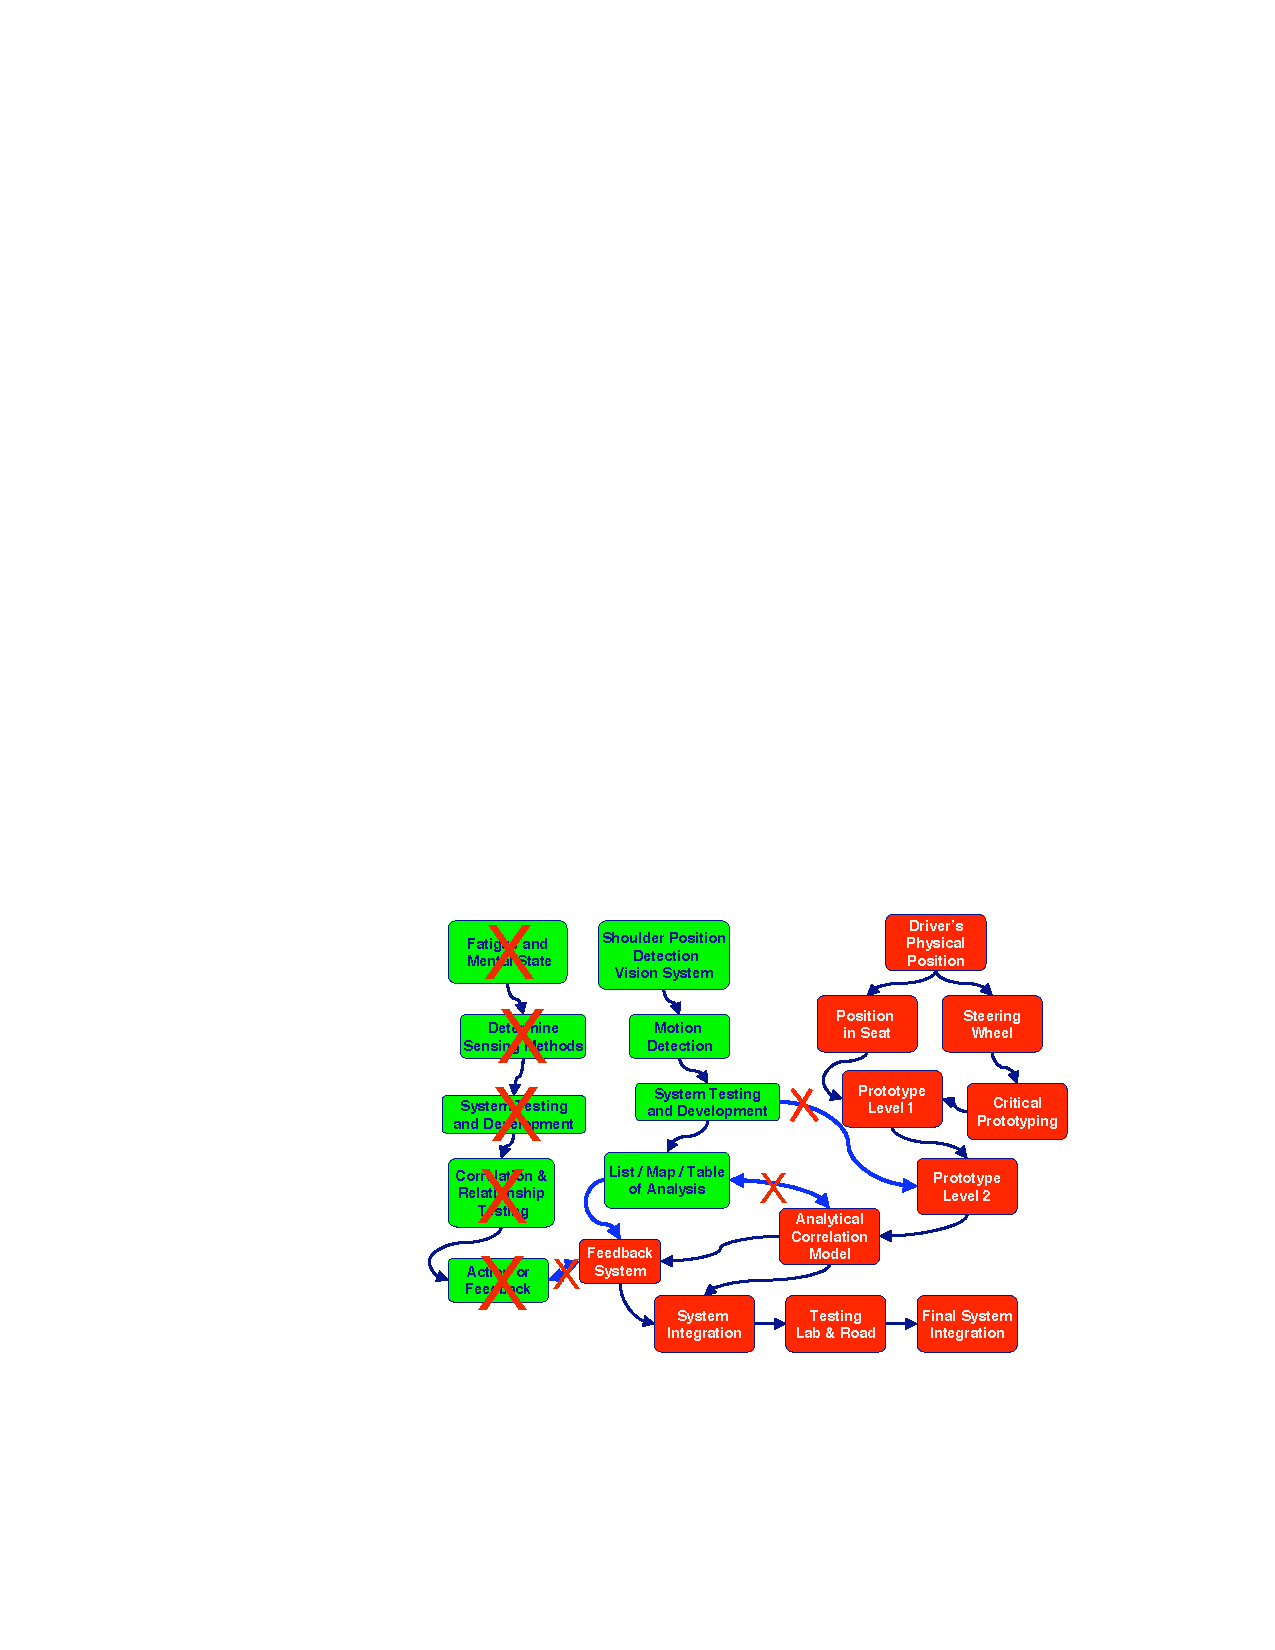
\includegraphics[width=\textwidth]{Figures/Ch6/su-tmit-after.pdf}
%         \caption[Project task replanning example]{In this example from \cite{Toyota01}, Stanford students collaborated with a group at TMIT, Japan. At the end of the Winter quarter it was decided to abandon one branch of the TMIT effort and to eliminate some of the tight coupling that was originally envisioned. }
%         \label{fig:su-tmit}  %Tag for referring to figure in text.
% \end{figure}

% \begin{figure}[p]   % p for "page" for let it be a full page figure!
% \centering
%                 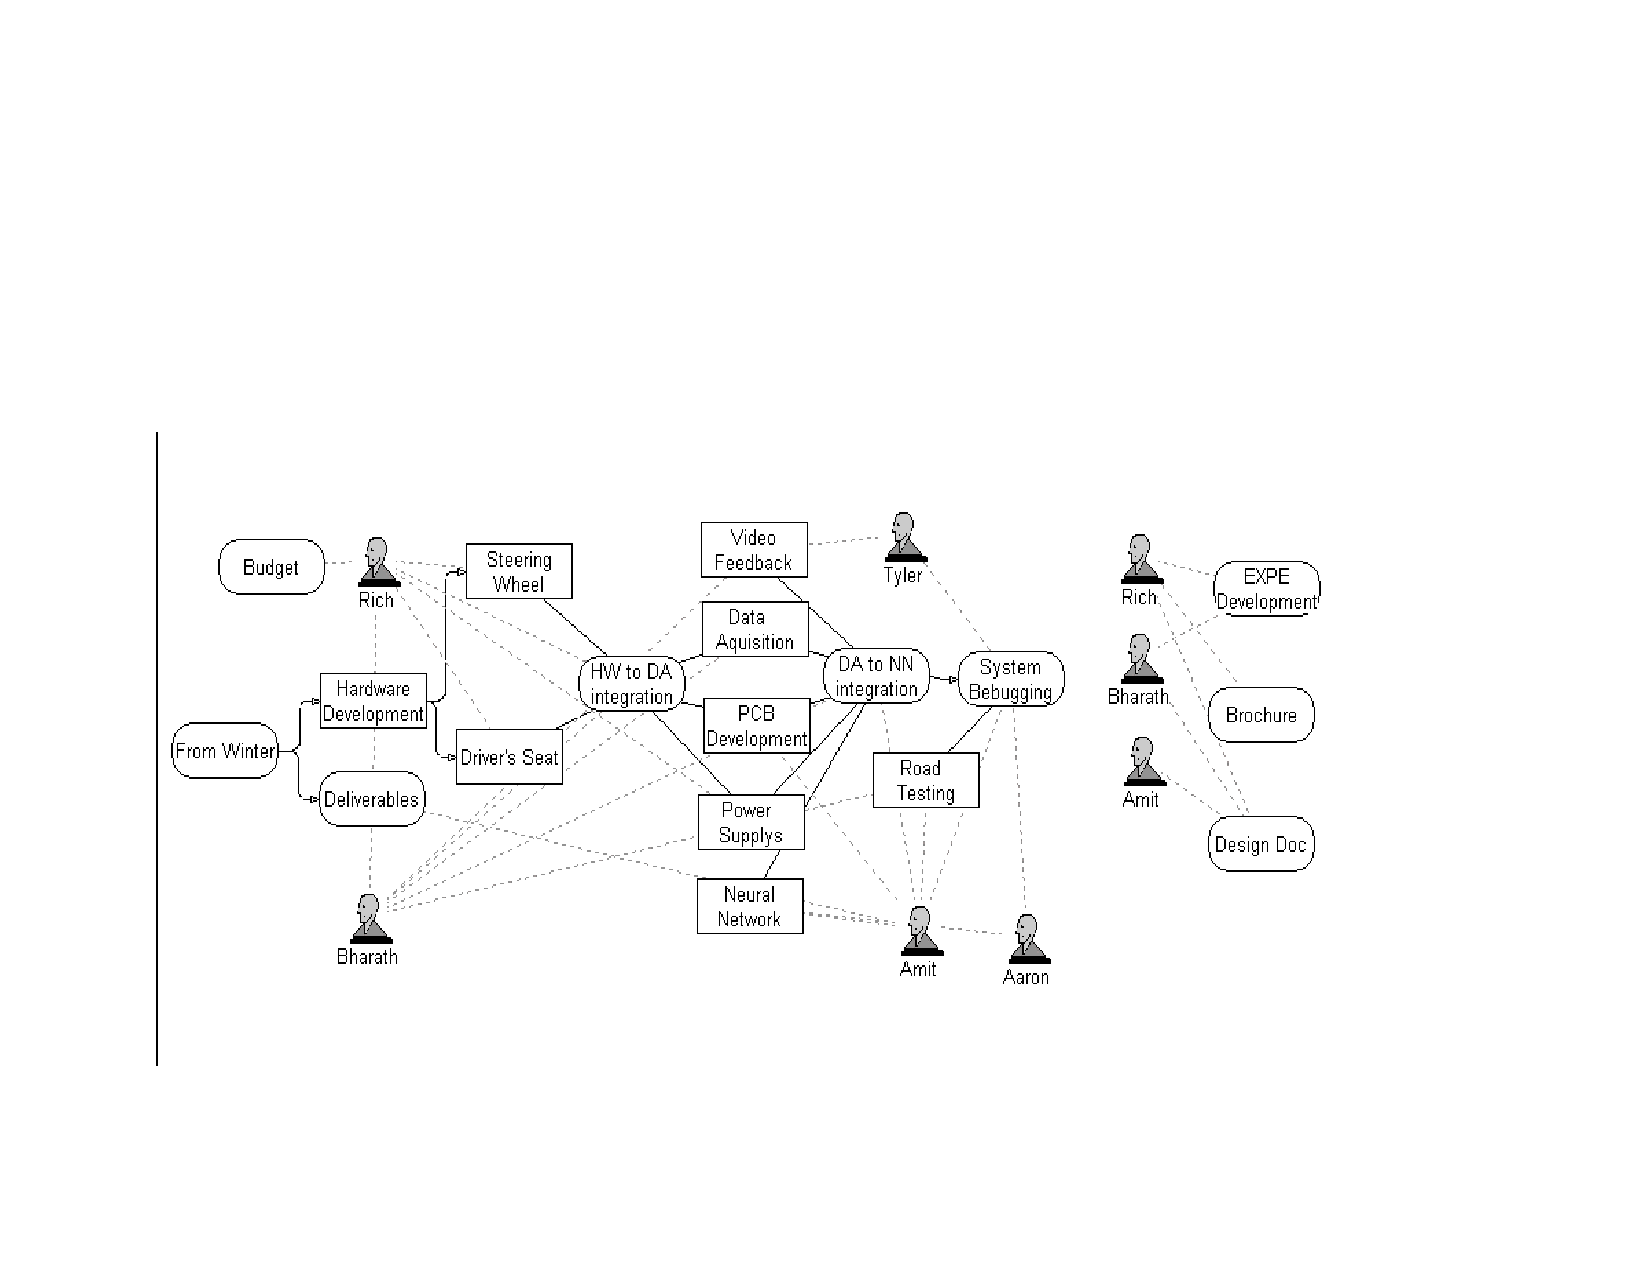
\includegraphics[angle=90, height= 8in]{Figures/Ch6/ideastorm}
%         \caption[Rotated landscape figure example]{An example of taking a large figure and having Latex rotate it 90 degrees to display it in landscape format as a full page figure.}
%         \label{fig:full-page-example}  %Tag for referring to figure in text.
% \end{figure}

\section{项目管理}
%Explain how your distributed and interdisciplinary team will collaborate, communicate and keep itself on-track with respect to the afore-mentioned deliverables.

本项目的前半期,我们采取了去中心的分布式的方法。文档系统被部署到网页可访
问的mediawiki上,文件的共享通过匿名ftp实现。后半期会加强分布式的管理方法,包括公开的git服务器,提供源代码版本控制和在线浏览;
公开的bugtracker,接受内部和外部的软件缺陷汇报并用于跟踪开发进度。

\section{经费结算}
%As with any serious proposal, you should include an estimated budget with some specifics about money that has been spent (Fall) and probably will be spent (Winter). Details on vendors can be put in the Appendix.

前半期使用经费800-900¥,留给之后的项目进展经费比较充足。

\section{思考和目标}
% This is the one section that you would not find in normal research or engineering proposal. But in the spirit that we're doing this in an academic setting, we want to be sure that we reflect on what we're learning and thinking and where we hope to go with it.

% A part of this may include how your team functioned in the fall - explaining how and why your actual design process deviated from what you originally planned, if relevant. (Time lines and milestones often have the look of having been concocted the night before the report is due.)
在前半期的设计中走了一些弯路,比如需求调查做的不充分,CFP的测试不够充
分等。主要原因还是人手不足和时间不够。所以在之后的工作中,一定要做好计划,充分
利用好时间。
